A \LaTeX{} file has a \verb|.tex| extension, and begins with a \emph{preamble}, where the document's \emph{class} is declared.
This is followed by a declaration to begin and end the \texttt{document} environment, with all of the document's contents being placed between these declarations, as can be seen below.

\begin{lstlisting}[caption=\texttt{example.tex}]
\documentclass[12pt]{article}
\begin{document}
    This is the first sentence of the first paragraph. Second sentence of first paragraph.
    Third sentence first paragraph.

    This is the second paragraph
\end{document}
\end{lstlisting}

Which when compiled produces the following output:
\begin{figure}[h]
    \centering
    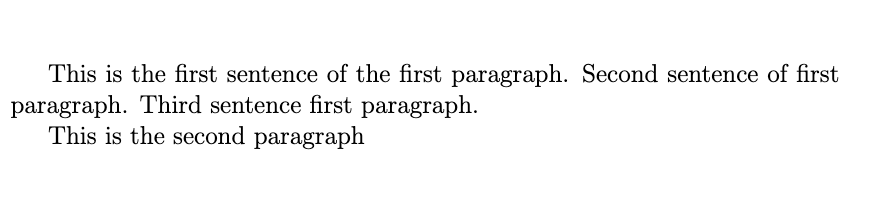
\includegraphics[width=0.8\textwidth]{figures/chapters.png}
    \label{fig:chapters}
\end{figure}

We declare a document class with \texttt{\textbackslash documentclass[option1, \ldots]\{class\}}, with the most commonly used classes being \verb|article| and \verb|report|.
Every class has a different set of default behaviours, such as \texttt{report} providing an automatic title page we will discuss later.
Generally default behaviour is good enough, but if you are curious, you can find more information on \href{https://texblog.org/2013/02/13/latex-documentclass-options-illustrated/}{this} link.

Default behaviours across \LaTeX{} can usually be modified by providing \emph{options}.
You can easily spot options, as they come between square brackets \verb|[]|.
The option in this example was to change the global font size from the default \verb|10pt| to \verb|12pt|.

Another option worth mentioning is \verb|twocolumn|, used to produce two column documents commonly seen in academia.
Try to recreate the example above with the addition of \verb|twocolumn| and see what it looks like.

Later on we will come back to the preamble for the inclusion of \emph{packages}, commands and other more complicated settings.
But bear in mind we tend to create templates to take care of them, so that regardless of how complicated a document's settings are, getting started is as easy as this example.

\subsection{Paragraph}
You will notice that the first paragraph consists of both lines 3 and 4.
This is because a paragraph is only created by having a full empty line (like line 5).
It is recommended that you do separate sentences with a new line, with the biggest advantage being that you can more easily move, copy and delete them in your editor.

Another important feature is that indentation is made automatically.
\LaTeX{} is smart enough to indent for you and almost always get it right.


\paragraph{Note:}
While it is possible to force a new line without indentation using \verb|\\|, like below, it is considered bad practice to do so in the context of normal text.
In fact, it will result in the common warning: \verb|Underfull hbox|.

This is nevertheless mentioned because \verb|\\| is how you correctly force a new line in matrices, text boxes in drawings and much more.
\begin{lstlisting}
    paragraph one\\
    paragraph two not indented.
\end{lstlisting}

\subsection{Font size}
Generally font size is changed globally for the document as shown before, but in some circumstances you may want to change the font size for a particular section. 
One example of how this can be done is the following:

\begin{lstlisting}
normal size text, followed by {\huge larger text}
\end{lstlisting}
normal size text, followed by {\huge larger text}

The use of brackets is very particular: \verb|{}| creates a limited scope, or in the other words, limits the font change to only the text inside the brackets.
Then \verb|\huge| scales the font relative to the global size.
The other font size options are:

\begin{table}[h]
\centering
\begin{tabular}{cc}
    Markup        & Example            \\ \hline
    \verb|\Huge        | &{\Huge Text}        \\
    \verb|\huge        | &{\huge Text}        \\
    \verb|\LARGE       | &{\LARGE Text}       \\
    \verb|\Large       | &{\Large Text}       \\
    \verb|\large       | &{\large Text}       \\
    \verb|\normalsize  | &{\normalsize Text}  \\
    \verb|\small       | &{\small Text}       \\
    \verb|\footnotesize| &{\footnotesize Text}\\
    \verb|\scriptsize  | &{\scriptsize Text}  \\
    \verb|\tiny        | &{\tiny Text}        
\end{tabular}
\label{tb:font-sizes}
\caption{Font size scaling}
\end{table}

\subsection{Quotations}
There are various ways to typeset quotations, but the standard in UK english is ``this'', which can be produced with: \texttt{\textasciigrave\textasciigrave text here\textquotesingle\textquotesingle}.
When you type each individual grave (\textasciigrave), the editor will automatically add the single quote (\textquotesingle).

\subsection{Bold, italic, underline, etc}
There are particular markups for each way text can be highlighted, as can be seen below. 

\begin{lstlisting}
\textit{Italics}, \underline{underline}, \textbf{bold}.
\textit{Emphasis switches from ``italics'' to \emph{normal}} and \emph{vice-versa} based on context.
\texttt{And we can even get monospace!}
\end{lstlisting}
% Results in: \\
\textit{Italics}, \underline{underline}, \textbf{bold}.
\textit{Emphasis switches from ``italics'' to \emph{normal}} and \emph{vice-versa} based on context.
\texttt{And we can even get monospace!}\\

While they are all quite verbose to type out, you generally use your editor to insert them in the same way you would use \keys{\ctrl+B} for bold in Word.
The shortcut for them in VSCode is as follows:
\keys{\ctrl+L} initiates a command, then \keys{\ctrl+B} creates the \textbf{b}old tag.
For Mac, just replace \keys{\ctrl} for \keys{\cmd}(\texttt{cmd}).

Similarly for the other highlights, use \keys{\ctrl + L} followed by:

\begin{table}[h]
\centering
\begin{tabular}{cc}
    Keys           & Shortcut              \\ \hline
    \keys{\ctrl+I} & \textit{Italics}      \\
    \keys{\ctrl+E} & \emph{Emphasise}      \\
    \keys{\ctrl+U} & \underline{Underline} \\
    \keys{\ctrl+T} & \texttt{Monospace}   
\end{tabular}
% \caption{Shortcut for highlighting with VSCode. Remember they are preceded by \keys{\ctrl+L}}
\end{table}

By pressing \keys{\ctrl+L+\ctrl+E} you create the markup \verb|\emph{}|, and it places the cursor between the brackets.
Alternatively you can select text, press the shortcut and it will place the markup around the selected text.

\paragraph{Note:} Generally the suggestion is to use \verb|\emph{}| over \verb|\textit{}|.
Think of it as a ``generic highlighter'' with default behaviour to \emph{italicise}, but you can modify it to change font colour, size or anything else.

\subsection{Sectioning}
Documents with the \texttt{article} class are primarily separated into \verb|section|, \verb|subsection|, \verb|\subsubsection| and \verb|paragraph|, with the first two showing up in a table of contents.
A \texttt{report} has, in addition to the above, \verb|\part| and \verb|\chapter|.

\begin{lstlisting}[caption=\texttt{example2.tex}]
\documentclass{article}
\begin{document}
    \tableofcontents
    \section{First header}
        text text.
        \subsection{Counted subheader}
            \paragraph{Leading text}
                normal text that follows.
        \subsection*{Uncounted subheader}
    \section{Second header}
\end{document}
\end{lstlisting}

Results in:
\begin{figure}[h]
    \centering
    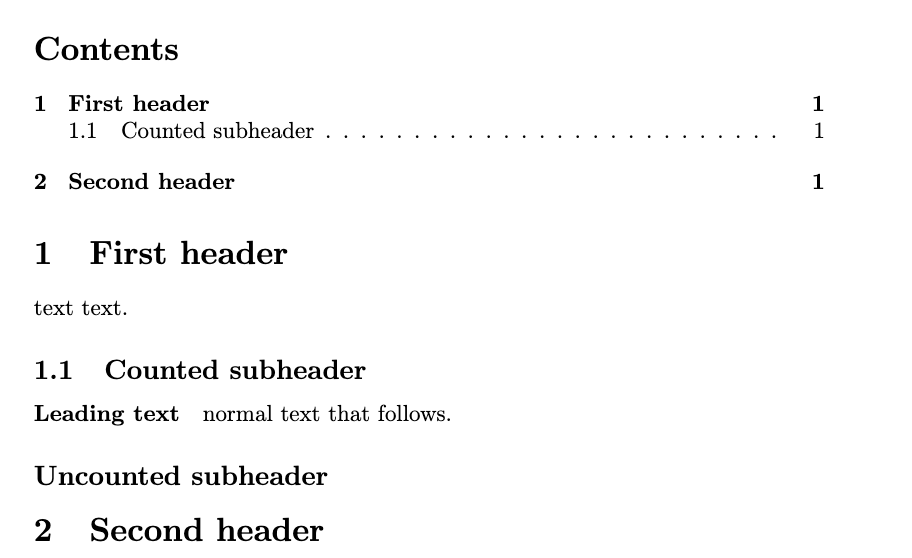
\includegraphics[width=0.6\textwidth]{figures/sections.png}
    \label{fig:sections}
\end{figure}

Every tag that includes some form of counting can have an asterisk (\verb|*|) to remove the counting.
In this case, you can see the difference between \verb|\section{}| and \verb|\section*{}|.
Most importantly, the table of contents --- generated with \verb|\tableofcontents| --- excluded the uncounted subheader.

\paragraph{Note:} You will notice that the table of content and the actual content are in the same page. If you want a page break at any point, just use \verb|\pagebreak|!

\subsection{Creating a title page}
By default only the classes \texttt{report} and \texttt{book} have a title page. To generate it, we declare an \verb|\author|, \verb|\title| and \verb|\date| in the preamble, then \verb|\maketitle| inside the \texttt{document} environment, like so:
\begin{lstlisting}
\documentclass{report}
\author{Jane Doe and John Smith}
\title{A seminal paper on cheese: \\ \large{exploring the deliciousness of Camembert} }
\date{01/01/1900}
\begin{document}
\maketitle
    Contents go here
\end{document}
\end{lstlisting}

Resulting in:
\begin{figure}[h]
\centering
    
\includegraphics[width=0.8\textwidth]{figures/title.png}
\label{fig:title}
\end{figure}

You can omit the date by leaving it empty, \verb|\date{}|, or automatically set it today with \verb|\date{\today}|.

An alternative that allows for a lot more customisation is to use the \texttt{titlepage} environment.
Overleaf has an excellent guide on it that can be found \href{https://www.overleaf.com/learn/latex/How_to_Write_a_Thesis_in_LaTeX_(Part_5):_Customising_Your_Title_Page_and_Abstract}{here}.